\documentclass[10pt]{beamer}

\usepackage[utf8]{inputenc}
\usepackage[german]{babel}
\usepackage{amsmath}
\usepackage{amsfonts}
\usepackage{amssymb}
\usepackage{tikz}
\usepackage{enumitem}
\usepackage{listings}
\usepackage{xcolor}
\usepackage[german,lined]{algorithm2e}
\usepackage{float}

\usetheme{Rochester}
\useinnertheme{rectangles}
\useoutertheme{default}

\lstset{
	basicstyle=\small\ttfamily,
	keywordstyle=\color{blue},
	showstringspaces=true}

\title{Probleme im Projektmanagement und Führungstipps}
\author{Oliver Erxleben}
\institute{Hochschule Osnabrück}
\date{\today}

\setitemize{label=\usebeamerfont*{itemize item}%
  \usebeamercolor[fg]{itemize item}
  \usebeamertemplate{itemize item}}

\begin{document}

	\thispagestyle{empty}
	\frame{\titlepage}
		
	\begin{frame}{Intro - Projektablauf}
		
	\end{frame}

	\begin{frame}{Intro - Projektbeteiligte}
	
		\begin{itemize}
			\item{Projektmitarbeiter}
			\item{Projektleiter}
			\item{Stakeholder}
		\end{itemize}

	
	\end{frame}
	
	\thispagestyle{empty}
	\frame{\centering{\textbf{Welche Faktoren beeinflussen den Projekterfolg?}}}
	
	\begin{frame}{Faktoren für Projekt(-miss-)erfolg}
		
		Eine Studie der GPM: Erfolg und Scheitern von 2008 erhob Daten aus: 
		\begin{itemize}
			\item{Befragung von 79 Unternehmen, mit hohem Anteil aus Mobilindustrie, Consulting, IT, Versicherung u. Bank }
			\item{überweigend Organisationen mit mehr als 1000 Mitarbeitern}
			\item{Erhebungsmethodik: über 30 Fragen an erfolgreiche und gescheiterte Projekte; jede Frage konnte dabei mit 1 (''trifft garnicht zu") und 5 (''trifft voll zu") beantwortet werden; Durchschnittswert einer Frage wurde erfolgreichem Projekt und gescheiterten Projekt gegenübergestellt}
		\end{itemize}

	\end{frame}

	\begin{frame}{Faktoren für Projekt(-miss-)erfolg 2}
	Ergebnis der Studie:
		\begin{center}
			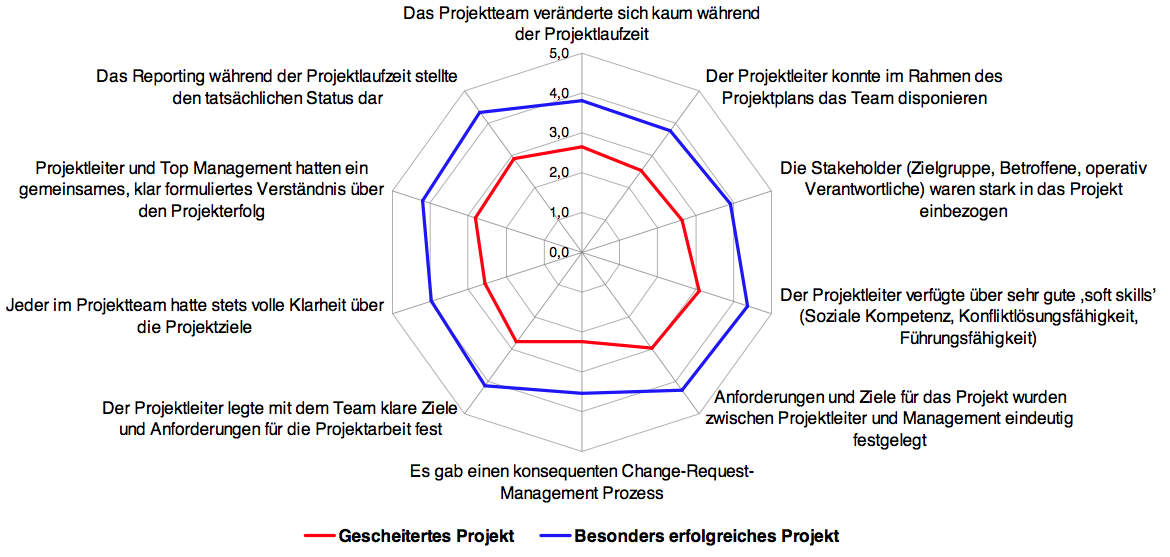
\includegraphics[width=1\textwidth]{images/studie_erfolgsfaktoren}
		\end{center}

	\end{frame}

	\begin{frame}{Faktoren für Projekt(-miss-)erfolg 3}
		Nach Gruppierung der Antworten, wurden folgende Top-5 Probleme festgestellt:
		\begin{itemize}
			\item{Kommunikation}
			\item{Klare Ziele}
			\item{Position des Projektleiters}
			\item{PM-Prozesse}
			\item{Teambesetzung}
		\end{itemize}

	\end{frame}
	
	\thispagestyle{empty}
	\begin{frame}
		''Der Widerspruch zwischen dem, was gesagt wird, und dem, was gemeint ist, ist sehr groß. Man muß ihn herausfinden.'' \\ 
		- \textit{Friedrich Eberling (Vorstandsvorsitzender Braun und Brunnen AG)}
	\end{frame}

	\begin{frame}{Probleme der Kommunikation}
		unterschiedliche Projektbeteiligte sprechen unterschiedliche Sprachen
	\end{frame}

	\thispagestyle{empty}
	\begin{frame}
		''Fleiß für die falschen Ziele ist noch schädlicher als Faulheit für die richtigen.'' \\
		- \textit{Peter Bamm (1897 - 1975, dt. Arzt u. Schriftsteller)}
	\end{frame}

	
	\begin{frame}{Problem der unklaren Projektziele}
		
	\end{frame}

	\thispagestyle{empty}
	\begin{frame}
		''Führen ist eine besondere Kategorie des Dienens.'' - Hans L. Merkle (1913-2000), dt. Topmanager, 1963-84 Vors. d. GF Bosch AG
	\end{frame}


	\begin{frame}{Problem der Karriestufe des PL}
		
	\end{frame}

	% TODO: Zitat finden
	\thispagestyle{empty}
	\begin{frame}
		
	\end{frame}

	
	\begin{frame}{Problem der Prozesse}
			
	\end{frame}
	
	\thispagestyle{empty}
	\begin{frame}
		„Teamwork = Wenn fünf Leute für etwas bezahlt werden, was vier billiger tun könnten, wenn sie nur zu dritt wären und zwei davon verhindert.“
Charles Saunders , Nähere Autorenangaben nicht feststellbar.
	\end{frame}

	
	\begin{frame}{Probleme im Team}
		
	\end{frame}

	\begin{frame}{Zusammenfassung}
		
	\end{frame}
	
	\begin{frame}{Quellen}
		
	\end{frame}

	\begin{frame}{FKK}
		\begin{itemize}
			\item{Fragen?}
			\item{Kommentare?}
			\item{Kritiken?}
		\end{itemize}

	\end{frame}



\end{document}